\section{METODOLOGI}

% Ubah konten-konten berikut sesuai dengan isi dari metodologi

\subsection{Metode yang digunakan}

Pada penelitian ini nantinya akan terdiri dari 2 langkah utama yaitu perancangan pada perangkat lunak (Softrware) dan perancangan pada perangkat keras (Hardware) :
%\begin{figure}[H]
%	\centering
%	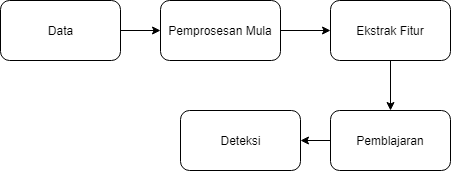
\includegraphics[width=\linewidth]{bab3/BlokDiagram}
%	\caption{Blok Diagram Penelitian}
%	\label{fig:blokdiagram}
%\end{figure}

\subsubsection{Perangkat Lunak}

\begin{figure}
	\centering
	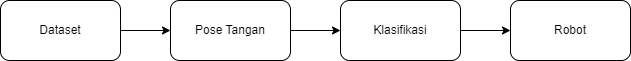
\includegraphics[width=1\linewidth]{gambar/gambar3.1}
	\caption{Blok Diagram Perangkat Lunak}
	\label{fig:Gambar 3.1}
\end{figure}

\subsubsubsection{Dataset}
Pada tahapan dataset disini akan dilakukan mulai dari pengambilan data-data yang disini nantinya akan berupa gambar/citra sampai dengan menyeleksi gambar tersebut dan siap melanjutkan ke tahapan selanjutnya.

\paragraph{Input Citra}
Pada dasarnya untuk mendeteksi suatu pose atau gerakan dari tangan membutuhkan untuk menemukan bagian tangan pada setiap Frame dan kemudian menganalisa pose atau gerakan tangan tersebut. Kamera digunakan untuk mendapatkan pose dari tangan pada setiap frame yang akan digunakan oleh user sebagai input untuk menentukan perintah. Dari input kamera ini yang nantinya akan digunakan untuk mendeteksi adanya tangan pada frame menggunakan Mediapipe.

\paragraph{Pose Estimation}
Mediapipe pada tangan memiliki 21 titik keypoint pada tangan. Setiap keypoint memiliki atribut posisi x, y, dan z. Data dari setiap titik yang nantinya akan diolah untuk menentukan gerakan dari tangan. Data koordinat dari setiap keypoint yang telah di dapatkan akan dilakukan normalisasi. Koordinat yang telah didapatkan merupakan koordinat dari setiap titik terhadap titik nol citra. Maka diperlukan perubahan dimana  koordinat setiap titik dirubah menjadi terhadap titik 0 keypoint. Jadi setiap ada perubahan posisi pada tangan masih dapat terukur posisinya terhadap titik 0 keypoint. Untuk jarak antar keypoint akan di scaling menggunakan jarak titik 0 ke titik 5 untuk menangani masalah dekat atau jauhnya tangan dari kamera. Untuk sudut pada tangan akan ada 3 titik dimana dianggap tidak bisa berotasi atau memilki sudut 0° yaitu pada titik 0, 5, dan 17. Data-data yang terlah dinormalisasi ini yang akan kemudian di simpan untuk dapat dideteksi.

\paragraph{Pose Extraction}
Hasil dari pendeteksian tangan menggunakan mediapipe akan diletakkan pada citra berwarna hitam.dan kemudian disimpan.

\subsubsubsection{Pose}


\subsubsubsection{Classification}
Data yang sudah didapatkan nantinya akan di inputkan ke dalam perhitungan menggunakan machine learning. Data yang telah diinputkan nantinya akan dilabeli untuk ada diklasifikasikan dan digunakan untuk memberikan action selanjutnya. Dari hasil kalsifikasi nantinya akan disimpan sebagai model yang nantinya akan digunakan untuk mendeteksi citra yang akan datang

\subsubsubsection{Action}
Dari data yang telah di klasifikasikan dan sudah didapatkan gesturnya maka gestur tersebut akan diterjemahkan ke dalam suatu perintah untuk dapat menggerakkan mobil robot.

\subsubsection{Perangkat Keras}

\begin{figure}
	\centering
	\includegraphics[width=0.7\linewidth]{"gambar/gambar perangkat keras"}
	\caption{Blok Diagram Perangkat Keras}
	\label{fig:gambar-perangkat-keras}
\end{figure}

\subsubsubsection{Laptop}
Laptop disini nantinya akan digunakan untuk menjalankan program perangkat lunak yang telah dikembangnkan untuk dapat menklasifikasikan tangan yang terdeteksi dan juga kamera yang terdapat pada laptop ini juga yang nantinya akan digunakan sebagai input gambar/citra. 

\subsubsubsection{Bluetooth}

\subsubsubsection{Mobil}

\subsection{Bahan dan peralatan yang digunakan}

\lipsum[13]
\lipsum[3]

\subsection{Urutan pelaksanaan penelitian}

% Ubah tabel berikut sesuai dengan isi dari rencana kerja
\newcommand{\w}{}
\newcommand{\G}{\cellcolor{gray}}
\begin{table}[h!]
  \begin{tabular}{|p{3.5cm}|c|c|c|c|c|c|c|c|c|c|c|c|c|c|c|c|}

    \hline
    \multirow{2}{*}{Kegiatan} & \multicolumn{16}{|c|}{Minggu} \\
    \cline{2-17} &
    1 & 2 & 3 & 4 & 5 & 6 & 7 & 8 & 9 & 10 & 11 & 12 & 13 & 14 & 15 & 16 \\
    \hline

    % Gunakan \G untuk mengisi sel dan \w untuk mengosongkan sel
    Pengambilan data &
    \G & \G & \G & \G & \w & \w & \w & \w & \w & \w & \w & \w & \w & \w & \w & \w \\
    \hline

    Pengolahan data &
    \w & \w & \w & \w & \G & \G & \G & \G & \w & \w & \w & \w & \w & \w & \w & \w \\
    \hline

    Analisa data &
    \w & \w & \w & \w & \w & \w & \w & \w & \G & \G & \G & \G & \w & \w & \w & \w \\
    \hline

    Evaluasi penelitian &
    \w & \w & \w & \w & \w & \w & \w & \w & \w & \w & \w & \w & \G & \G & \G & \G \\
    \hline

  \end{tabular}
\end{table}
